%\textcolor{red}{\hrulefill \textsc{Unfinished Section}\hrulefill}  \\
\begin{figure}
    \centering
    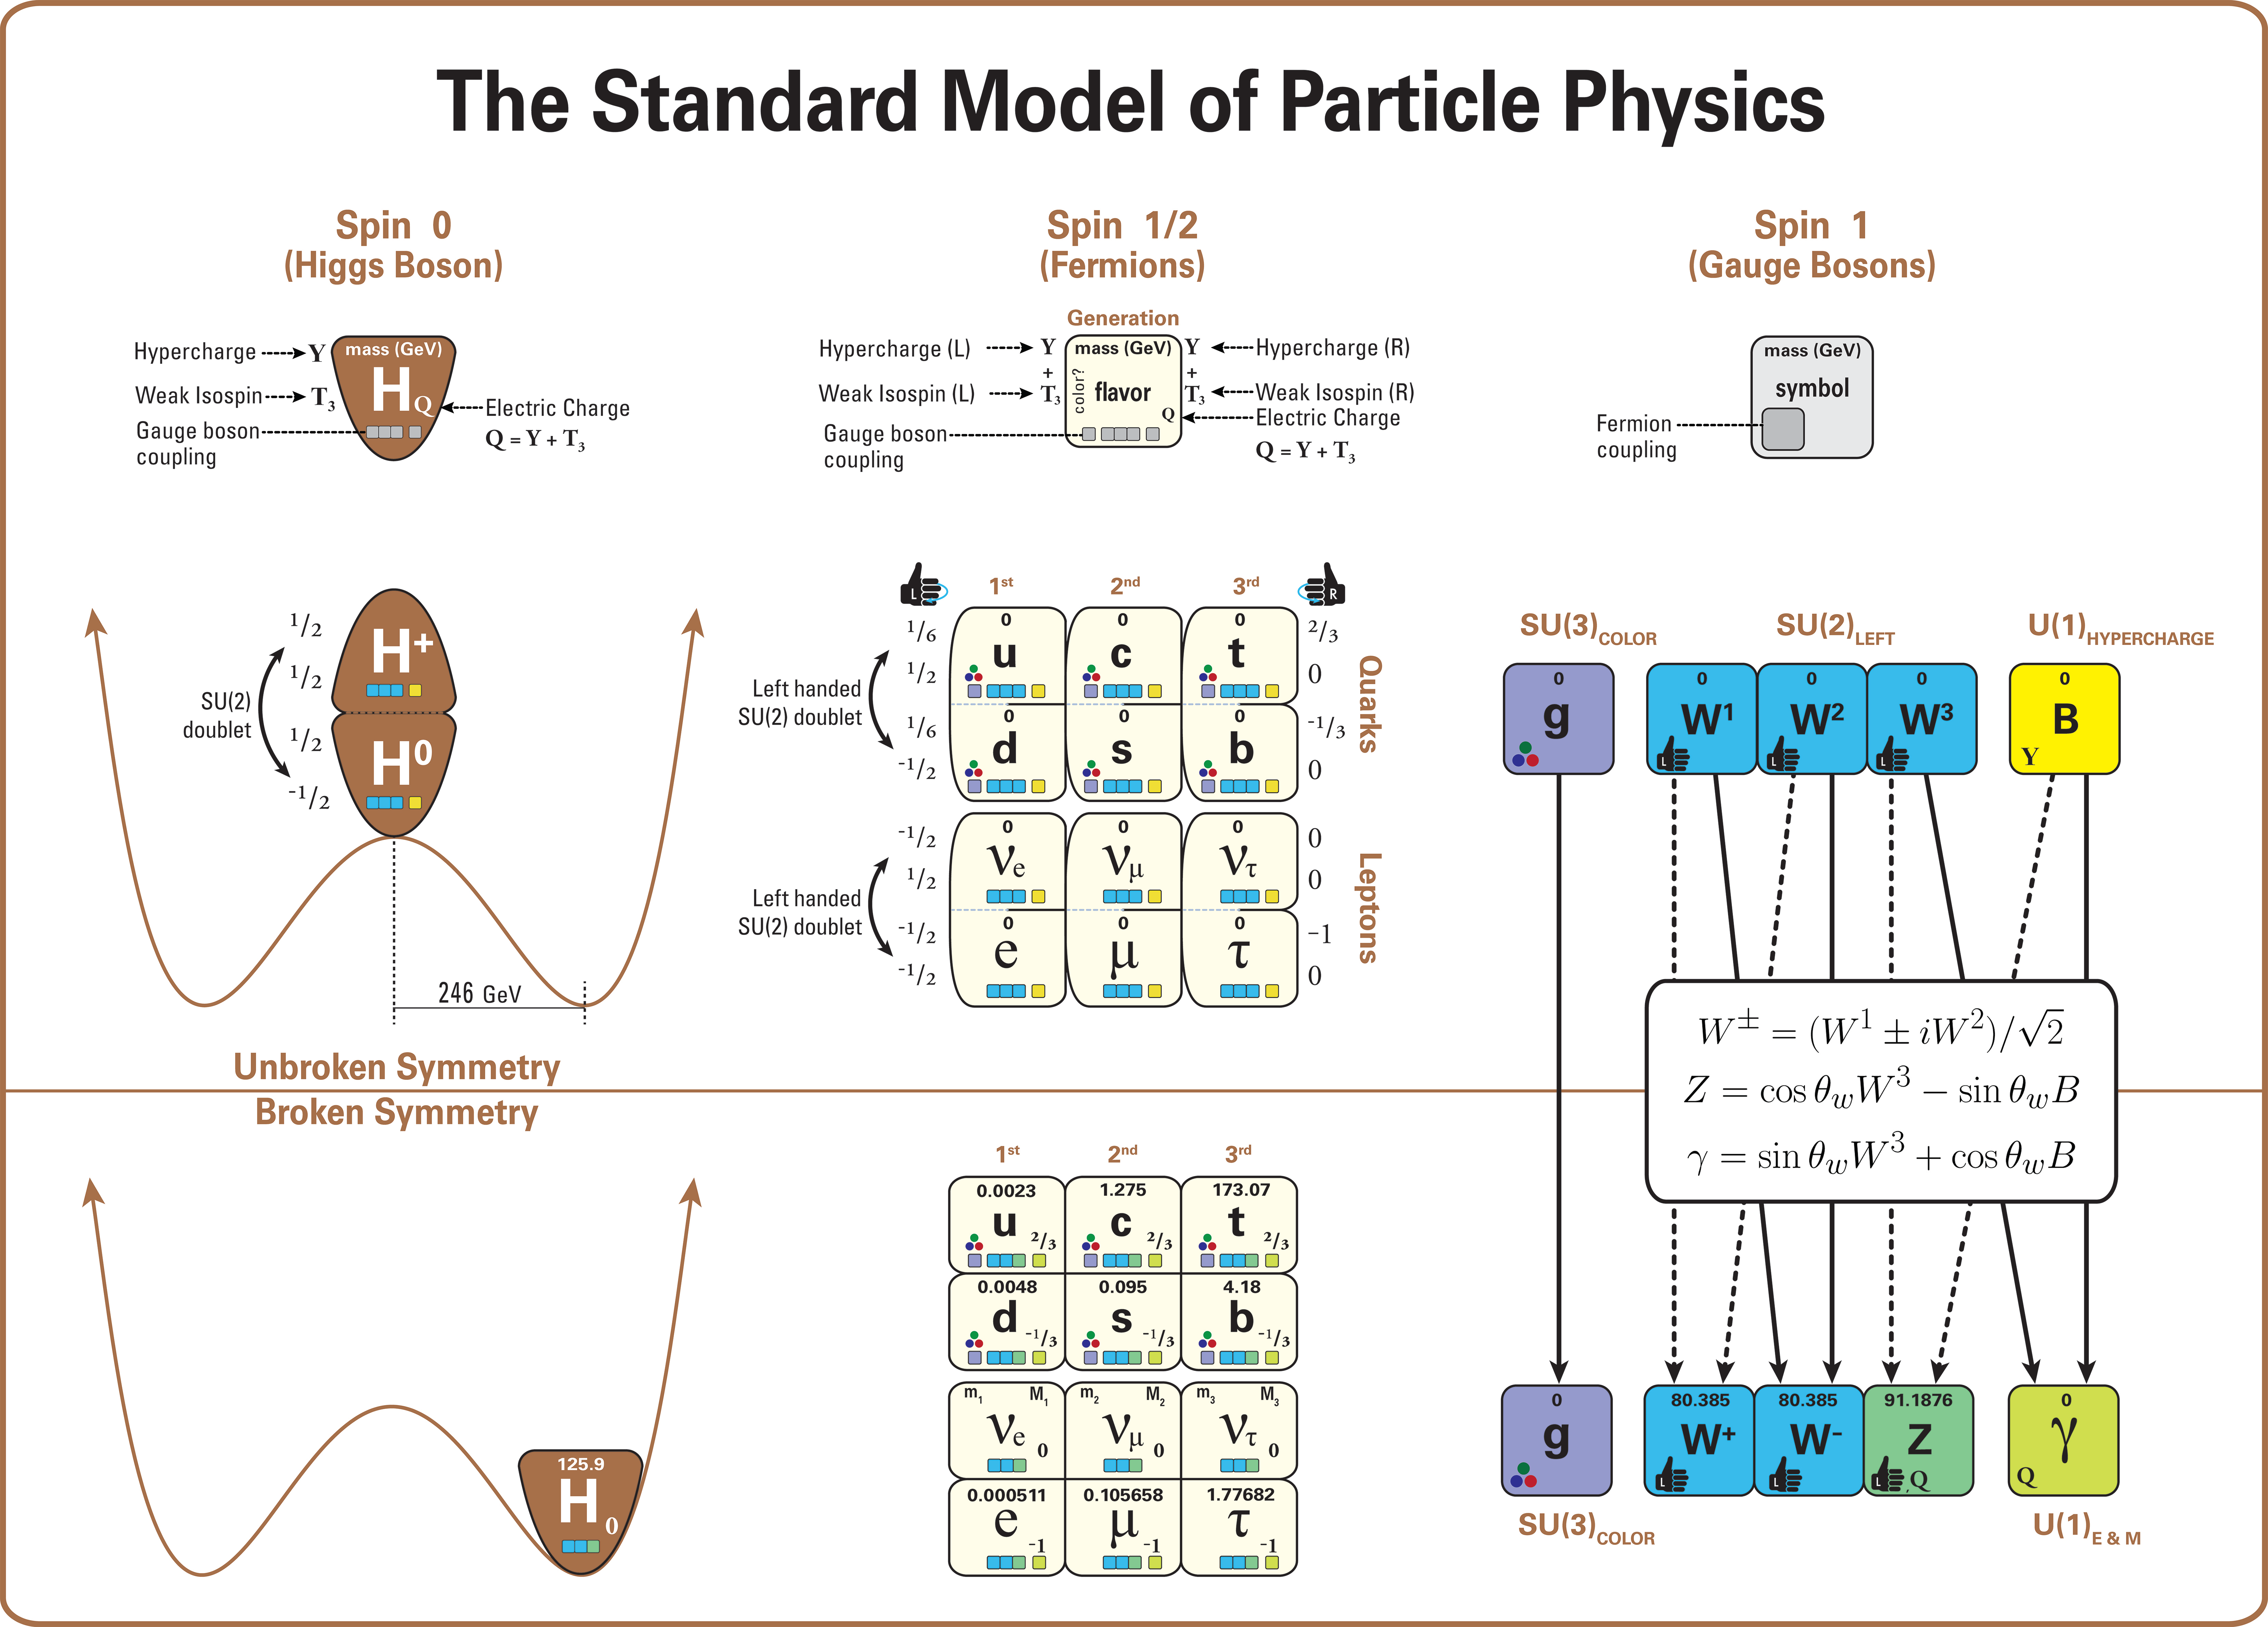
\includegraphics[width=0.90\textwidth]{figs/theory/Standard_Model_Of_Particle_Physics--Most_Complete_Diagram.png}
    \caption[Particle content of the Standard Model both before and after spontaneous symmetry breaking.
    Also shown is an illustration of spontaneous symmetry breaking via the Higgs Mechanism]{Particle content of the Standard Model both before and after spontaneous symmetry breaking.
    Also shown is an illustration of spontaneous symmetry breaking via the Higgs Mechanism~\cite{wiki:xxx}}
    \label{fig:theory:SM}
\end{figure}
Modern particle physics is generally interpreted in terms of the Standard Model (SM).
The SM is a QFT which encapsulates our understanding of the electromagnetic, weak, and strong interactions.
Noticeably missing of course is the force of gravity, which is described by Einstein's General Relativity (GR). 
Theories that reconcile GR and QFT belong to a topic that would take up it's own library and shall not be discussed further as Gravity is so comparably small for our experiments in particle physics that it has no measurable effect and can be easily ignored.
The SM obeys a set of symmetries such that the theory belongs the gauge unitary product group 
\begin{equation}
    SU(3)_{C} \times SU(2)_{L} \times U(1)_{Y}
\end{equation}

\subsection{Quantum Chromodynamics}\label{sec:theory:QCD}
$SU(3)_{C}$ is the gauge symmetry group for the theory of the strong force, Quantum Chromodynamics (QCD), which defines the strong interaction between quarks and gluons.
The strong force is mediated by the force carrying gluons, which each carry the color charges (red, green, blue) and anti-color charges (anti-red, anti-green, anti-blue), leading to a total of 9 possible states of gluons.
However the special color singlet state, which would be indicative of a long range force like the photon, is not observed in nature and so only 8 physical color states are possible.
Gluon-gluon interactions constrain the color fields to string-like objects called ``flux tubes'', so that as two quarks are pulled apart there is a binding energy that increases linearly with their separation.
At a large enough distance, it becomes energetically more favorable to pull a quark-antiquark pair out of the vacuum rather than increase the length of the flux tube.
A phenomenon known as color confinement, this has a cascading effect of the two very energetically separating quarks pulling quark-antiquark pairs out of the vacuum along their journey (which also in turn can do the same), thereby forming hadrons is known as hadronization.
This is an experimentally confirmed phenomenon showing up in particle detectors as large conical sprays or \emph{jets} of particles.

\subsection{Electroweak Unification}\label{sec:theory:ewkuni}
$SU(2)_{L}\times U(1)_{Y}$ is the gauge group for the theory of the Electroweak force.
At high energies, the well known electromagnetic force and the weak nuclear force are unified into a single electroweak force.
Composed of the four massless gauge vector bosons $W_{1},W_{2}, W_{3} $ from the weak isospin ($T$) field and $B$ from the weak hypercharge ($Y$) field, the $SU(2)$ Higgs doublet, and the nominal three generations of charged and neutral fermions.
The particle content for this theory is illustrated in the upper half of Figure~\ref{fig:theory:SM}.

\subsection{Spontaneous Symmetry Breaking and the Higgs Mechanism}
We however do not live in a world with these particles - a very good thing or nuclear fusion reactions and radioactive decays would run much faster and stars and humans would not exist at all!
We say that this electroweak symmetry is broken, and the Higgs mechanism was proposed as an explanation that was confirmed 40 years later with the discovery of the Higgs boson in 2012 by the ATLAS and CMS experiments at CERN.
The Higgs mechanism occurs when any charged field (the Higgs field) at some critical temperature acquires a vaccuum expectation value (vev) which induces spontaneous breaking of three out of four generators of $SU(2)_{L}\times U(1)_{Y}$ 
Due to electroweak symmetry breaking, the neutral boson from weak isospin and the hypercharge boson mix to form two different states: the massless photon that is the force carrier of the electromagnetic force; and the massive \Zboson\ boson that is the neutral current of the weak force.
The other two weak isospin bosons form the massive \Wplus and \Wminus bosons that carry the electrically charged current of the weak force.
The ratio of the \Wboson\ and \Zboson\ boson masses is predicted by the theory, as are the couplings of the \Zboson\ boson to quarks and leptons.
These are experimentally confirmed to high precision.
%The SM symmetry group can then be written as 
%\begin{equation}
%   SU(3)_{C} \times SU(2)_{} \times U(1)_{}
%\end{equation}
%Where $SU(2)$ and $U(1)$ are the familiar weak and electromagnetic forces respectively.
Figure~\ref{fig:theory:SM} diagrammatically shows this symmetry breaking and the boson mixing that gives us the particle content that we observe in the world we live in today and is seen in the bottom half of the Figure. 

\subsection{The Standard Model Lagrangian}
The full SM Lagrangian is as follows
\begin{equation}
     \mathcal{L}_{SM} = -\frac{1}{4}F_{\mu\nu}F^{\mu\nu} + i\bar{\psi}{D\!\!\!\!/}\psi  + h.c. +  \psi_{i}y_{ij}\psi_{j}\phi + h.c. + |D_{\mu}\phi|^{2} - V(\phi)
\end{equation}
Where some terms look familiar from our QFT exercises in Appendix~\ref{app:qft} and others not so much.
It is useful here to break this down term by term.
\begin{enumerate}
    \item $-\frac{1}{4}F_{\mu\nu}F^{\mu\nu}$:  This term is the scalar product of the field strength tensor $F_{\mu\nu}$ which contains the mathematical encoding of all force carrying interaction particles except the Higgs boson.
    \item $i\bar{\psi}{D\!\!\!\!/}\psi$: This term describes how these interaction particles interact with matter particles.
    The fields $\psi$ and $\bar{\psi}$ describe (anti)quarks and (anti)leptons
    \item $h.c.$: This term represents the ‘hermitian conjugate’ of the second term.
    The hermitian conjugate is necessary if arithmetic operations on matrices produce complex-valued ‘disturbances’.
    By adding h.c., such disturbances cancel each other out, thus the Lagrangian remains a real-valued function.
    \item $\psi_{i}y_{ij}\psi_{j}\phi $: This term describes how matter particles couple to the Higgs field $\phi$ and thereby obtain mass.
    The entries of the Yukawa matrix $y_{ij}$ represent the coupling parameters to the Higgs field, and hence are directly related to the mass of the particle in question.
    These parameters are not predicted by theory, but have been determined experimentally.
    \item $h.c.$: See term 3, but here this term is really necessary, since term 4 is not self-adjoint.
    \item $|D_{\mu}\phi|^{2}$: This term describes how the interaction particles couple to the Higgs field.
    \item $-V(\phi)$: This term describes the potential of the Higgs field. 
    Contrary to the other quantum fields, this potential does not have a single minimum at zero but has an infinite set of different minima.
    This makes the Higgs field fundamentally different and leads to spontaneous symmetry breaking.
\end{enumerate}

%The Electroweak symmetry $SU(2)_C \times U(1)_{Y}$ is broken via the \emph{Higgs Mechanism}, which is essential in explaining how mass is generated for gauge bosons. 
%\subsection{Quantum Electrodynamics}\label{sec:theory:QED}
%\textcolor{red}{\hrulefill \textsc{Unfinished Section}\hrulefill}\\
%\subsection{The Weak Interaction}\label{sec:theory:weak}
%\textcolor{red}{\hrulefill \textsc{Unfinished Section}\hrulefill}\\

